% !TEX root = thesis.tex
\documentclass[12pt,a4paper,titlepage,listof=totoc,bibliography=totoc,chapteratlists=0pt]{scrreprt}
\begin{filecontents*}{\jobname.xmpdata}
	\Keywords{CHANGEME, VR, IOT, TODO}
	\Title{CHANGEME: Unser tolles Thema -- wir sind suppa}
	\Author{CHANGEME, Stefan Schwammal, Susi Schwammal}
\end{filecontents*}

\setcounter{tocdepth}{1}

\usepackage[utf8]{inputenc}
\usepackage[T1]{fontenc}
\usepackage{amsmath}
\usepackage{amsfonts}
\usepackage{amssymb}
\usepackage[table]{xcolor}
\usepackage{graphicx}
\usepackage[left=3.50cm, right=2.00cm, top=2.00cm, bottom=2.00cm,foot=1cm]{geometry}
\usepackage[splitrule,hang,flushmargin,multiple,bottom]{footmisc}
\usepackage{lmodern, textcomp}
\usepackage{lmodern}
\usepackage{pdfpages}
\usepackage[ngerman]{babel}
\usepackage{multicol}
\usepackage{float}
\usepackage{array,tabularx,booktabs}
\usepackage{ragged2e}
\usepackage{lipsum}
\usepackage{wrapfig}

\newcolumntype{M}[1]{>{\centering\arraybackslash}m{#1}}

\usepackage{enumitem}
\newlist{compactitem}{itemize}{3}
\setlist[compactitem,1]{label=\textbullet, nosep,leftmargin=1.5em,labelwidth=*,align=left}
\setlist[compactitem,2]{label=--, nosep,leftmargin=1.5em,labelwidth=*,align=left}
\setlist[compactitem,3]{label=\textopenbullet, nosep,leftmargin=1.5em,labelwidth=*,align=left}
\newlist{compactenum}{enumerate}{3}
\setlist[compactenum,1]{label=\arabic*., nosep,leftmargin=1.5em,labelwidth=*,align=left}
\setlist[compactenum,2]{label=\alph*., nosep,leftmargin=1.5em,labelwidth=*,align=left}
\setlist[compactenum,3]{label=\roman*., nosep,leftmargin=1.5em,labelwidth=*,align=left}
\newlist{compactdesc}{description}{3}
\setlist[compactdesc]{leftmargin=1.5em,labelwidth=*,align=left}

\usepackage{microtype}

\usepackage[parfill]{parskip}

\definecolor{bluekeywords}{rgb}{0.13,0.13,1}
\definecolor{greencomments}{rgb}{0,0.5,0}
\definecolor{redstrings}{rgb}{0.9,0,0}
\definecolor{lightgray}{gray}{0.9}
\definecolor{lightblue}{rgb}{0.93,0.95,1.0}

\usepackage{listings}

\makeatletter
\lstdefinestyle{lststyle}{
	basicstyle=%
	\ttfamily
	\lst@ifdisplaystyle\scriptsize\fi
}
\makeatother

\renewcommand{\lstlistlistingname}{List of Listings}
% TODO: define other languages as needed
\lstset{language=Python,
numbers=left,               
numberstyle=\tiny,          
showspaces=false,
showtabs=false,
breaklines=true,
lineskip=-1pt,
tabsize=2,
showstringspaces=false,
breakatwhitespace=true,
escapeinside={(*@}{@*)},
commentstyle=\color{greencomments},
keywordstyle=\color{bluekeywords}\bfseries,
stringstyle=\color{redstrings},
style=lststyle,
xleftmargin=17pt,
         framexleftmargin=17pt,
         framexrightmargin=5pt,
         framexbottommargin=4pt
}
\lstset{
morekeywords={base,var,in,out,dynamic,from,where,select,orderby,function,\$,group,by,into,yield,async,await,@,None,self,as,elif,with}
}
\lstdefinelanguage{TypeScript}{
	keywords={typeof, new, true, false, catch, function, return, null, switch, var, if, in, while, do, else, case, break, void, number, string, boolean, module, \$, export, for, this},
	keywordstyle=\color{blue}\bfseries,
	ndkeywords={class, export, boolean, throw, implements, import, this},
	ndkeywordstyle=\color{darkgray}\bfseries,
	identifierstyle=\color{black},
	sensitive=false,
	comment=[l]{//},
	morecomment=[s]{/*}{*/},
	commentstyle=\color{purple}\ttfamily,
	stringstyle=\color{red}\ttfamily,
	morestring=[b]',
	morestring=[b]"
}
\usepackage{caption}
\DeclareCaptionFont{white}{\color{white}}
\DeclareCaptionFormat{listing}{\colorbox[cmyk]{0.43, 0.35, 0.35,0.01}{\parbox{\textwidth}{\hspace{10pt}#1#2#3}}}
\captionsetup[lstlisting]{format=listing,labelfont=white,textfont=white} 
\captionsetup[table]{justification=centering, singlelinecheck=false}

\usepackage{subcaption}

\usepackage{setspace}
\newcommand{\MSonehalfspacing}{%
	\setstretch{1.44}%  default
	\ifcase \@ptsize \relax % 10pt
	\setstretch {1.448}%
	\or % 11pt
	\setstretch {1.399}%
	\or % 12pt
	\setstretch {1.433}%
	\fi
}

\newcommand{\setauthor}[1]{\ohead[]{#1}}

\usepackage[automark]{scrlayer-scrpage}
\pagestyle{scrheadings}
\automark{chapter}
\renewcommand\sectionmark[1]{\markright{\MakeMarkcase {\thesection\hskip .5em\relax#1}}}
\rohead{\ifnum\expandafter\pdfstrcmp\botmark=0 \rightmark\else\leftmark{} --- \rightmark\fi}
\ihead[]{\headmark}
\chead[]{}
\ohead{}
\cfoot[]{}
\ofoot[\pagemark]{\pagemark}
\setheadsepline{.1pt}

\usepackage[hyphens]{url}

\usepackage[a-1b]{pdfx}

\usepackage{hyperref}
\hypersetup{pdfa}

\usepackage[nonumberlist,toc,nopostdot]{glossaries}

\usepackage{chngcntr}
\counterwithout{footnote}{chapter}
\counterwithout{figure}{chapter}
\counterwithout{table}{chapter}
\AtBeginDocument{
	\counterwithout{lstlisting}{chapter}
	\urlstyle{sf}
}
\newcounter{RPages}

\makeatletter
\def\bstctlcite{\@ifnextchar[{\@bstctlcite}{\@bstctlcite[@auxout]}}
\def\@bstctlcite[#1]#2{\@bsphack
	\@for\@citeb:=#2\do{%
		\edef\@citeb{\expandafter\@firstofone\@citeb}%
		\if@filesw\immediate\write\csname #1\endcsname{\string\citation{\@citeb}}\fi}%
	\@esphack}
\makeatother

\clubpenalty=10000 
\widowpenalty=10000
\displaywidowpenalty=10000
\interfootnotelinepenalty=10000

\title{Anmeldeformular Unterstützung für das Sekretariat}
\author{Dominik Ortbauer}

\makeindex
\makeglossaries
\begin{document}
\bstctlcite{IEEEexample:BSTcontrol}
\newcommand{\reminder}[1]
{ \textcolor{red}{<[{\bf\marginpar{\mbox{$<==$}} #1 }]>} }
\newcommand{\icode}[1]{\lstinline$#1$}
%\urlstyle{same}
%\setstretch{1.5}
\setstretch {1.433}
\renewcommand{\arraystretch}{1.2}


\includepdf{./titlepage/coversheet}
\pagenumbering{Roman}
\newpage
\thispagestyle{empty}
\vspace{3cm}
~ \\ \\
Ich erkläre an Eides statt, dass ich die vorliegende Diplomarbeit selbstständig und ohne fremde Hilfe verfasst, andere als die angegebenen Quellen und Hilfsmittel nicht benutzt bzw. die wörtlich oder sinngemäß entnommenen Stellen als solche kenntlich gemacht habe.

Die Arbeit wurde bisher in gleicher oder ähnlicher Weise keiner anderen Prüfungsbehörde vorgelegt und auch noch nicht veröffentlicht.

Die vorliegende Diplomarbeit ist mit dem elektronisch übermittelten Textdokument identisch.
\vspace{3cm}
% Hier kommt die Unterschrift drüber
\begin{tabbing}
Leonding, September 2023 \hspace{5cm} D. Ortbauer
\end{tabbing}
\vspace{10cm}
\newpage
\setcounter{page}{1}

\begin{spacing}{1}
    \chapter*{Abstract}
\end{spacing}
\begin{wrapfigure}{r}{0.3\textwidth}
    \begin{center}
      
\includegraphics[width=0.2\textwidth]{pics/question_mark.png}
    \end{center}
\end{wrapfigure}
Brief summary of our amazing work. In English.
This is the only time we have to include a picture within the text.
The picture should somehow represent your thesis.
This is untypical for scientific work but required by the powers that are.
\lipsum[6]
\newpage
\begin{spacing}{1}
    \chapter*{Zusammenfassung}
\end{spacing}
\begin{wrapfigure}{r}{0.3\textwidth}
    \begin{center}
      
\includegraphics[width=0.2\textwidth]{pics/question_mark.png}
    \end{center}
\end{wrapfigure}
Zusammenfassung unserer genialen Arbeit. Auf Deutsch.
Das ist das einzige Mal, dass eine Grafik in den Textfluss eingebunden wird.
Die gewählte Grafik soll irgendwie eure Arbeit repräsentieren.
Das ist ungewöhnlich für eine wissenschaftliche Arbeit aber eine Anforderung der Obrigkeit.
\emph{Bitte auf keinen Fall mit der Zusammenfassung verwechseln, die den Abschluss der Arbeit bildet!}
\lipsum[6]


\pagestyle{plain}

\renewcommand{\lstlistlistingname}{Quellcodeverzeichnis}

\tableofcontents
\newpage
\setcounter{RPages}{\value{page}}
\setcounter{page}{0}
\pagenumbering{arabic}
\pagestyle{scrheadings}

\begin{spacing}{1}
\chapter{Introduction}\label{chapter:introduction}
\end{spacing}
\lipsum[2-3]

\begin{spacing}{1}
\chapter{Related Work}
\end{spacing}
\lipsum[4] Citing \cite{InfH} properly.

Was ist eine \gls{guid}?
Eine \gls{guid} kollidiert nicht gerne.

Kabellose Technologien sind in abgelegenen Gebieten wichtig \cite{APCW2006}.


\begin{spacing}{1}
\chapter{Technologies}\label{chapter:tech}
\end{spacing}
%\section{Foo}
%\setauthor{Stefan Schwammal}
%\lipsum[5-12]

%\section{Bar}
%\setauthor{Susi Schwammal}
%\lipsum[12-18]

%\subsection{Deeper}
%Nicht mehr im Inhaltsverzeichnis.

%\subsubsection{Deepest}
%Vermeide mich.

\section{React Native}
React native allows for the development of cross platform mobile applications using javascript/typescript and the react framework.
For this project React Native was chosen as the framework for the mobile application
because of the author's experience with typescript as well as its cross platform compatability
which is important because the school staff does not have a uniform phone operating system.

\subsection{Expo}
Expo was used as a development environment for its ease of use and quick development cycle.
Expo allows you to use your own phone to test your application without the need for an emulator like Android Studio.
It also enables the easy use of the camera via the expo-camera package which was especially useful for this project.

\section{Visual Studio Code}
The author used Visual Studio code as his editor of choice for this project because it was set up very quickly without any complications.

\section{Communication}
The communication between the document understanding model running os a flask server and the mobile application is done via WebSockets
because the model needs to accept incoming images of the application form and return the extracted data for validation.

Was kann man da alles noch dazu schreiben? Access? Programming language?

\begin{spacing}{1}
\chapter{Alternate Solutions}\label{chapter:tech}
\end{spacing}
\section{Robotic Process Automation}
\setauthor{Dominik Ortbauer}

When looking at the problem of this project, the first thought for solving it is to use some sort of Robotic Process Automation like UiPath or Power Automate.

RPA uses software robots to automate tedious and menial digital tasks. This is done by programming these robots to do the exact same things a human would do such as moving the mouse and typing data into textboxes using the keyboard. 

Said robots are especially useful when automating tasks that require moving data between different applications. The other option, creating an interface, would be a lot more work or simply not possible if you can not alter the code for both applications.

It is important to understand the limits of Robotic Process Automation. While it excels at rule based decisions and repetitive tasks it struggles with complex decisions and changing environments.
AI can help with some of these problems but can not remove these restrictions entirely.

RPA is never the best way to solve a problem and always just a transitional solution. However, it is way cheaper than the alternatives as well as faster to develop and therefore it is widely used.

Digital robots can do the same job faster, more efficient and more reliable than humans and they are also easily scalable. They can also employ techniques which humans can not do such as accessing a REST API or talking to programs directly without the user interface.

\cite{RPAFundamentals}

One way to create a RPA solution is to use UiPath.

\subsection{UiPath}
\setauthor{Dominik Ortbauer}

UiPath consists of three major components: UiPath Studio which is used by the developers to program the robots, the robots which execute the workflows developed in said Studio and the Orchestrator as a central hub where the code gets published to and jobs are assigned to robots.

\subsubsection{UiPath Studio}
Developers use UiPath Studio to write the instructions for the robots. For example, when a workflow needs to log into a web app the developer uses two "type into" commands to type in the username and password and one "click" to click the submit button. 

UiPath Studio also offers more advanced features like Computer Vision, Data Scraping and Document Understanding.

\subsubsection{UiPath Robot}
A robot interacts with the software and performs all the tasks as described in the workflow created in UiPath Studio.

There is a differentiation between tasks that interact with a user interface (attended automation) and tasks that can be performed without using any UI (unattended automation). 
Unattended processes are used for automating back office jobs and more scalable than their counterparts used for front office jobs.

\subsubsection{UiPath Orchestrator}
The Orchestrator is the web application where it all comes together. The workflows created in UiPath Studio get published to here and jobs can be scheduled or run immediately from this web app.

It also allows for the administration of assets used to store data that can be accessed by the robots as well as queues allowing for a convenient scalable producer - consumer pattern implementation. Another feature of the Orchestrator is the user management which includes licence allocation.

\begin{figure}
    \centering
    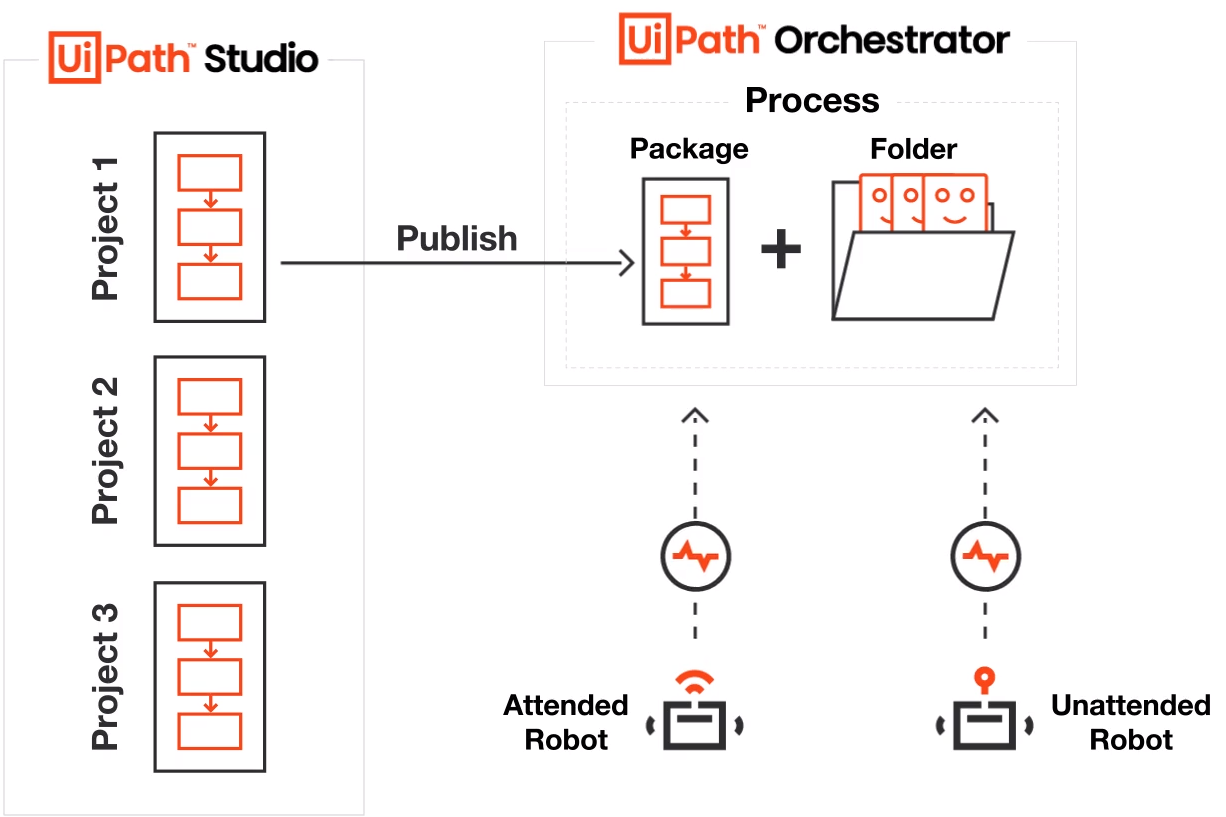
\includegraphics[scale=0.4]{pics/UiPathArchitecture.png}
    \caption{Studio, Robot and Orchestrator Architecture}
    \label{fig:as:UiPathArchitecture}
\end{figure}

\cite{UiPathOverview}
\cite{UiPathAcademyOverview}

Due to budgeting reasons UiPath was not used for this project seeing as it requires a licence for commercial use. Aside from than that, it would be a good solution for this kind of problem due to UiPaths Document Understanding capabilities and the automation features required for inserting the data into the database.

\subsection{Power Automate}
\setauthor{Dominik Ortbauer}

Power Automate is a digital automation tool developed by Microsoft and formerly known as Microsoft Flow. Workflows are created in the web and then scheduled or triggered to run. Examples for this include running a workflow on the first of every month which backs up a server and using a trigger to run one every time an email is received and then classifying it according to the emails subject.

Power Automate offers connectors for all Microsoft 365 apps and countless more which enables you to connect them. You can for example receive an email and then upload it to SharePoint in order to archive it. If no connectors fit your need it also offers the possibility to create your own.

The tool is aimed at people with no coding experience and therefore is very simple to use. There is a predefined set of actions that can be used to do almost everything. This includes conditions, loops and other logic as well as the communication with apps like SharePoint, Outlook, GMail, Dropbox and many more. Again, if there is an action missing you can create it yourself.

\cite{PowerAutomateOverview}

Power Automate was not used for this project because it does not innately offer Document Understanding which is a vital part of this project and the other parts            do not contain enough automation possibilities to justify using an external software.

\section{Digital Application Form}
\setauthor{Dominik Ortbauer}

Another possibility to achieve the goal of this project would be to digitize the application form. In order to make this happen a web page would need to be created with all the values from the application form.

Security would be very important for this project due to it containing a lot of personal data. Some sort of validation would be needed so that unfinished entries can not be submitted and the same person can not submit an application twice.

The backend of this digital application form would be almost the same as the backend for this project except for the Document Understanding part which would not be necessary. It would only enter the data into the access database with optional validation in between.

This is a good approach to the problem but the paper version of the application form is not going to disappear and therefore an automation of both versions is ideal.

This project aims to automate only the paper version of the application form but there is another diploma thesis which focuses on creating a digital version of the application form.


\begin{spacing}{1}
\chapter{Implementation}\label{chapter:implementation}
\end{spacing}
Siehe tolle Daten in Tab. \ref{tab:impl:data}.

\begin{table}
    \centering
    \begin{tabular}{|lcc|}
    \hline
              & \textbf{Regular Customers} & \textbf{Random Customers} \\ \hline
    Age       & 20-40                      & \textgreater{}60          \\ \hline
    Education & university                 & high school               \\ \hline
    \end{tabular}
    \caption{Ein paar tabellarische Daten}
    \label{tab:impl:data}
\end{table}

\begin{figure}
    \centering
    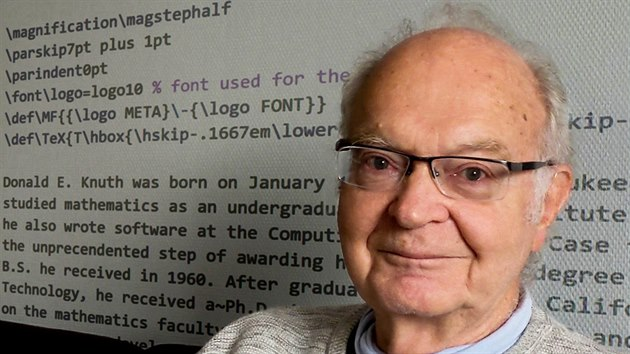
\includegraphics[scale=0.5]{pics/knuthi.jpg}
    \caption{Don Knuth -- CS Allfather}
    \label{fig:impl:knuth}
\end{figure}

Siehe und staune in Abb. \ref{fig:impl:knuth}.
\lipsum[6-9]
Dann betrachte den Code in Listing \ref{lst:impl:foo}.

\begin{lstlisting}[language=Python,caption=Some code,label=lst:impl:foo]
# Program to find the sum of all numbers stored in a list (the not-Pythonic-way)

# List of numbers
numbers = [6, 5, 3, 8, 4, 2, 5, 4, 11]

# variable to store the sum
sum = 0

# iterate over the list
for val in numbers:
    sum = sum+val

print("The sum is", sum)
\end{lstlisting}

\begin{spacing}{1}
\chapter{Summary}
\end{spacing}
Aufzählungen:

\begin{compactitem}
    \item Itemize Level 1
    \begin{compactitem}
        \item Itemize Level 2
        \begin{compactitem}
            \item Itemize Level 3 (vermeiden)
        \end{compactitem}
    \end{compactitem}
\end{compactitem}

\begin{compactenum}
    \item Enumerate Level 1
    \begin{compactenum}
        \item Enumerate Level 2
        \begin{compactenum}
            \item Enumerate Level 3 (vermeiden)
        \end{compactenum}
    \end{compactenum}
\end{compactenum}

\begin{compactdesc}
    \item[Desc] Level 1
    \begin{compactdesc}
        \item[Desc] Level 2 (vermeiden)
        \begin{compactdesc}
            \item[Desc] Level 3 (vermeiden)
        \end{compactdesc}
    \end{compactdesc}
\end{compactdesc}

\newpage
\pagenumbering{Roman}
\setcounter{page}{\value{RPages}}
\newacronym{guid}{GUID}{Globally Unique Identifier}
\newacronym{jit}{JIT}{Just In Time Compiler}
\newacronym{nfc}{NFC}{Near Field Communication}
\newacronym{rfid}{RFID}{Radio Frequency Identification}

% Usage:
% \gls{label} lowercase in text
% \Gls{label} Uppercase in text
% \newacronym{label}{abbrev}{full}
% \newglossaryentry{label}{settings}



%\setlength{\glsdescwidth}{0.8\linewidth}
\glsnogroupskiptrue
\printglossary[title=Glossary,toctitle=Glossary] %,style=long]
\spacing{1}{
%\bibliographystyle{IEEEtran}
\bibliographystyle{ieeetrande}
\bibliography{bib}
}
\listoffigures
\listoftables
\lstlistoflistings
\appendix
\addchap{Appendix}
\input{./sections/appendix}
\end{document}

